\documentclass[11pt,a4paper]{article}
\usepackage[margin=1in]{geometry}
\usepackage{iftex}
\ifPDFTeX
  \usepackage{times}
\else
  \usepackage{fontspec}
  \setmainfont{Times New Roman}
\fi
\usepackage{amsmath,amssymb}
\usepackage{booktabs}
\usepackage{array}
\usepackage{graphicx}
\usepackage{tikz}
\usepackage{xcolor}
\usetikzlibrary{arrows.meta,positioning,fit,calc}
\usepackage{placeins}
\usepackage{float}
\usepackage{algorithm}
\usepackage{algpseudocode}
\usepackage{framed}
\colorlet{shadecolor}{black!4}
\usepackage{hyperref}
\usepackage[numbers]{natbib}

\title{Adapting Tool Documentation for Cross-Hop Parameter Passing}
\author{%
Sergey Bugaev\\
ITMO University, Saint Petersburg\\[0.85em]
{\small Advisor: Stanislav Batalenkov}%
}
\date{14 September 2026}

\begin{document}
\maketitle

\begin{abstract}
Language agents can be asked to solve multi-hop questions by calling REST APIs, given only the vendor catalog as documentation. Those catalogs are written for humans: they name the next endpoint and leave implicit which previous call yields a path identifier and which fields in a list payload are stubs. The model then invents an id, the call is rejected, and the trace still looks well-formed. We study which documentation slot of a released depth-first controller should carry that binding. We compile fill and response contracts from the catalog and a handful of live probes, and write them into those slots. A fill contract names the producer call and the JSON path of each path parameter; a response contract names the returned fields and the hops those identifiers feed. The object is the slot, not a learned rewriter. On RestBench-TMDB, replicated on Ling and DeepSeek V4, a fill line in the guideline is more executable than a free-form purpose rewrite on both families. Against the original catalog it wins on Ling and matches on DeepSeek V4, while the free-form rewrite fails on both.
\end{abstract}

\section{Introduction}

To answer a multi-hop REST question (retrieve a collection, read the movie list, fetch a review), the agent is given only the vendor catalog as documentation~\cite{song2023restgpt,qin2024toollm}. Toolformer, ReAct, and Gorilla already show that a language model can emit a search query, a calculator call, or an API name~\cite{schick2023toolformer,yao2023react,patil2024gorilla}. Pointed at that catalog, the same idea still depends on what the catalog says.

That catalog is written for a human reader. Each entry names a purpose and a URL template. It does not say which earlier call produces the identifier that belongs in the template, or which keys in a list payload are real fields rather than stubs. The model is left to invent the binding. On a live backend the invention is cheap to detect: the path parameter is missing or wrong, HTTP rejects the call, and the trace can still contain every gold API name.

Existing edits of the same documents rarely target that binding as a fill slot. DRAFT rewrites the purpose paragraph from trial feedback~\cite{qu2025draft}; EasyTool compresses a vendor page into a short instruction~\cite{yuan2025easytool}. Both change the purpose slot; the guideline read after the hop is chosen stays a human sentence. Trace-Free+ learns a description rewriter and, on RestBench, scores it under teacher forcing~\cite{guo2026tracefree}. Arazzo and OpenAPI Links already write a producer path as a workflow spec~\cite{arazzo2024}. AutoRestTest and APIPilot recover producer--consumer edges to generate tests, not to fill an existing DFSDT catalog~\cite{kim2025autoresttest,nguyen2026apipilot}. Gorilla, Toolformer, ReAct, and ToolGen change the model, the index, or the prompting loop~\cite{patil2024gorilla,schick2023toolformer,yao2023react,wang2025toolgen}. The write we study is a typed producer path in the fill slot of a catalog that already exists.

Figure~\ref{fig:teaser} shows that binding failure on one RestBench-TMDB query. The user asks for a review of a movie from a named collection. Search finds the collection, but the review endpoint still needs a movie identifier. Under the vendor catalog the collection id is filled and the movie id is left as a stub: the live call is rejected and there is no review. Under DRAFT both stubs stay empty. Under the compiled fill contract the controller writes the correct id from the collection parts list, and HTTP returns a user review.

\begin{figure}[ht]
\centering
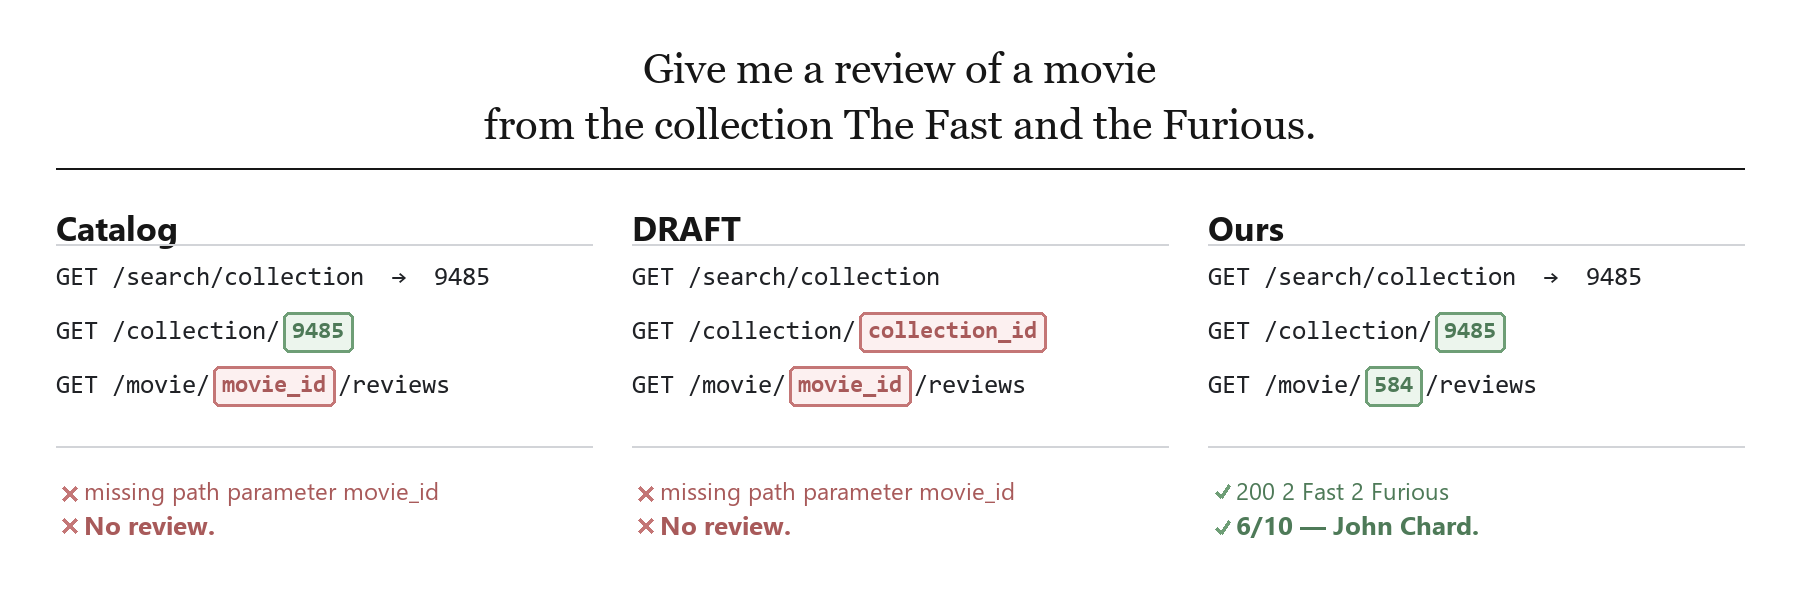
\includegraphics[width=\textwidth]{figures/teaser.png}
\caption{The same RestBench-TMDB query under three documents. Catalog and DRAFT emit the review hop and leave the movie id unbound; the live call is rejected and there is no review. The fill contract writes the correct id from the collection parts list and returns a user review.}
\label{fig:teaser}
\end{figure}

We compile two short contracts from the catalog and a handful of live probes, without gold paths. A \emph{fill} contract on every hop API names the producer calls and the JSON path of each path parameter. A \emph{response} contract on every search or list API names the returned fields and the downstream hops those identifiers feed. Both go into the documentation slots of a released depth-first controller~\cite{qin2024toollm}, leaving the search procedure and the request schema as they are.

The edit is a typed line in the fill slot, not a rewrite of the purpose sentence. Fill is kept out of the selection surface of hop APIs, because extra text there makes the agent repeat search and skip the id call; response scope is compressed on catalog tools only. The same sentence in another slot is a different intervention.

The rest of the paper evaluates that slot write on RestBench against the vendor catalog and against DRAFT, on a live TMDB backend and two model families. The tables, like Figure~\ref{fig:teaser}, score whether the last hop executes. Agreement with gold API names can stay high in every arm. Where the same payload helps one family and blocks another, that limit belongs to the edit, not to a new generator of descriptions.

\section{Related work}

\subsection*{REST agents}
RestGPT connects a language model to live vendor REST APIs and releases RestBench: multi-hop questions on TMDB and Spotify, scored as an ordered path against gold \texttt{relevant APIs}~\cite{song2023restgpt}. We keep those queries and that gold list. A gold name sequence can still fail HTTP, so we also score whether every call on the path is accepted by the live backend. ToolLLM's DFSDT controller searches a catalog depth-first~\cite{qin2024toollm}. \texttt{choose\_tool} reads a purpose $u_t$; \texttt{choose\_parameter} reads a guideline $d_t$. We use the released driver and change only the strings in those slots.

\subsection*{Models, indexes, and prompting loops}
Toolformer trains a language model to insert API calls into its own generations~\cite{schick2023toolformer}. Gorilla finetunes a model to write API calls and retrieves documentation at inference~\cite{patil2024gorilla}. ReAct interleaves a reasoning trace with an action~\cite{yao2023react}. ToolGen represents each of tens of thousands of APIs as a vocabulary token and trains retrieval and calling as next-token prediction on ToolBench~\cite{wang2025toolgen}. Intra-collection splits already require one call's output to become another call's input; the training target is still the API name, and the catalog strings stay as found. Each of these changes how the model is trained, indexed, or prompted.

\subsection*{Purpose-slot rewrites}
DRAFT lets a model explore an API and rewrites the purpose paragraph from trial feedback~\cite{qu2025draft}. EasyTool compresses a vendor page into a short instruction~\cite{yuan2025easytool}. Both write on the selection surface. The fill slot, read after the hop is chosen, stays the human guideline shipped with the catalog. DRAFT released a RestBench rewrite; that dump is the documentation baseline in the tables.

Trace-Free+ learns a description generator and evaluates it on RestBench TMDB and Spotify as out-of-domain tools~\cite{guo2026tracefree}. The generator emits one description per tool. Their protocol supplies the gold API at each subtask and executes that API, so a later step never has to bind a path id after the agent itself chose the hop. DFSDT does not run that way: \texttt{choose\_tool} reads $u_t$, \texttt{choose\_parameter} reads $d_t$, and the live backend can reject a missing id. A single rewritten description has no fill slot. Copied into hop $u_t$, extra bind text makes the agent repeat search (Section~\ref{sec:placement}); copied into both slots, it is a purpose rewrite in the guideline, which is the DRAFT row. The criterion we score is a typed producer path that is visible only after the hop is chosen, on live HTTP. That is a two-slot write under a released controller, not a teacher-forced one-field rewriter.

\subsection*{Producer--consumer edges outside the agent}
AutoRestTest builds a semantic property graph over OpenAPI and uses live responses to fill later test requests~\cite{kim2025autoresttest}. APIPilot treats inferred producer--consumer edges as hypotheses and keeps an edge only after a live injection succeeds~\cite{nguyen2026apipilot}. That loop is close to our Bind and Probe steps. Both papers generate tests; they do not write a fill line into DFSDT's guideline. Arazzo and OpenAPI Links already name a producer path in a workflow spec, for example \texttt{\$response.body\#/id}~\cite{arazzo2024}. The RestBench dump has no such links. The agent we study reads natural-language slots, not an Arazzo runtime.

\subsection*{Wrappers and retrieval fields}
Doc2Agent compiles documentation into executable wrappers~\cite{ni2025doc2agent}. The agent then talks to those wrappers, not to the original catalog strings. MFTR standardizes document fields so a retriever can rank tools~\cite{tang2026mftr}. Ranking decides which tool page is fetched. The failure in Figure~\ref{fig:teaser} is later: the review hop is already chosen, and the movie id is still unbound. The write we study is a fill line on every hop API and a response line on every search or list API, in the purpose and guideline slots DFSDT reads at those two steps.

\FloatBarrier
\section{Method}

\subsection{Notation and scoring}
\label{sec:setup}

The input is a finite vendor catalog $\mathcal{T}$. Each tool $t$ is four strings the released DFSDT driver splits across prompts: a purpose $u_t$ (read by \texttt{choose\_tool}), a guideline $d_t$ (read by \texttt{choose\_parameter}), a request schema $\theta_t$, and a URL template $p_t$. Path parameters $\phi(p_t)$ are the placeholders in that template, such as \texttt{movie\_id} in \texttt{/movie/\{movie\_id\}/reviews}. Closed enumerations (\texttt{media\_type}, \texttt{time\_window}) are not treated as identifiers.

An agent $\pi$ maps a user query $q$ and a document set $D$ to a call sequence $a_{1:m}$. RestBench ships, for each query, a gold list $g_{1:k}$ of API names. The ordered-path score counts that list as a correct path if and only if the names appear in order as a subsequence of $a_{1:m}$. The score does not look at arguments. Execution-valid CP adds a second check: no call on that path was rejected by the live backend because a path parameter was missing or invented. A cell that still carries a harness error after the driver's own resample is dropped from $n$, not scored as a miss.

Let $E$ be the closed set of enumeration parameters $\{\texttt{media\_type},\texttt{time\_window},\texttt{type}\}$. Tool $t$ is a \textbf{hop} if and only if $\phi(p_t)\setminus E\neq\emptyset$. Otherwise $t$ is a \textbf{catalog} tool: a search or list endpoint whose URL has no path identifier. The compiler (Algorithm~\ref{alg:compile}) reads $\mathcal{T}$ and writes a new document set $D^\star$. It does not read gold paths or evaluation traces. Figure~\ref{fig:method} states the four steps; Figure~\ref{fig:slots} shows the two DFSDT prompts after the write.

\begin{figure}[ht]
\centering
\resizebox{\textwidth}{!}{%
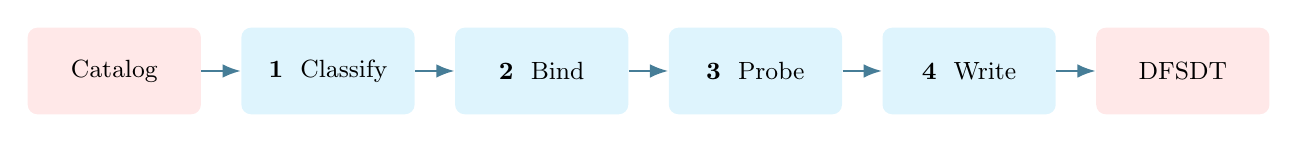
\begin{tikzpicture}[
  font=\small,
  endbox/.style={
    rounded corners=3.5pt, align=center, inner sep=6pt,
    minimum height=1.1cm, minimum width=2.2cm, fill=red!9
  },
  stepbox/.style={
    rounded corners=3.5pt, align=center, inner sep=6pt,
    minimum height=1.1cm, minimum width=2.2cm, fill=cyan!13
  },
  arr/.style={-{Latex}, thick, cyan!55!black}
]
\node[endbox] (cat) {Catalog};
\node[stepbox, right=0.5cm of cat] (c1) {\textbf{1}~~Classify};
\node[stepbox, right=0.5cm of c1] (c2) {\textbf{2}~~Bind};
\node[stepbox, right=0.5cm of c2] (c3) {\textbf{3}~~Probe};
\node[stepbox, right=0.5cm of c3] (c4) {\textbf{4}~~Write};
\node[endbox, right=0.5cm of c4] (out) {DFSDT};

\draw[arr] (cat) -- (c1);
\draw[arr] (c1) -- (c2);
\draw[arr] (c2) -- (c3);
\draw[arr] (c3) -- (c4);
\draw[arr] (c4) -- (out);
\end{tikzpicture}%
}

\vspace{0.75em}
{\small
\setlength{\tabcolsep}{4.5pt}
\begin{tabular}{@{}
  >{\raggedright\arraybackslash}p{1.7cm}
  >{\raggedright\arraybackslash}p{2.95cm}
  >{\raggedright\arraybackslash}p{2.95cm}
  >{\raggedright\arraybackslash}p{2.95cm}
  >{\raggedright\arraybackslash}p{2.95cm}
@{}}
\toprule
 & 1 Classify & 2 Bind & 3 Probe & 4 Write \\
\midrule
Hop API
  & URL template has a path parameter
  & closed map or name heuristic
  & seed then follow-up; drop stubs
  & fill line into $d_t$ \\[0.45em]
Catalog API
  & URL template has no path id
  & hops that consume a returned id
  & returned fields, not stubs
  & $R_t$ into $d_t$; scope into $u_t$ \\
\bottomrule
\end{tabular}}
\caption{Four compiler steps and what they write on a hop API versus a catalog API. The request schema is unchanged.}
\label{fig:method}
\end{figure}

\subsection{Compiler}
\label{sec:compiler}

Each $t$ enters Algorithm~\ref{alg:compile} as the vendor Initial dump $(u_t^0,d_t^0,\theta_t^0,p_t)$. Classify reads $\phi(p_t)\setminus E$. A hop receives a fill contract $F_t=\{(\alpha,S_\alpha,\ell_\alpha)\}_{\alpha\in\phi(p_t)\setminus E}$. A catalog tool, and a hop that itself emits further identifiers, receives a response contract $R_t=(\kappa_t,\Delta_t)$: the keys a list payload actually contains, and the hop APIs those identifiers feed. The write is
\begin{align}
d_t^\star &= d_t^0 \oplus F_t \oplus R_t, \label{eq:guideline}\\
u_t^\star &= u_t^0 \oplus \mathrm{scope}(R_t) \quad\text{on catalog tools only,} \label{eq:purpose}\\
\theta_t^\star &= \theta_t^0. \label{eq:schema}
\end{align}
$\oplus$ concatenates onto the vendor sentence. Fill is not written into hop $u_t$, so \texttt{choose\_tool} still sees the vendor purpose on those APIs. $\mathrm{scope}(R_t)$ is the compression in Section~\ref{sec:contracts}. On Spotify search, $\mathrm{scope}(R_t)$ is omitted.

\begin{algorithm}[H]
\caption{Compile fill and response contracts from a vendor catalog.}
\label{alg:compile}
\begin{algorithmic}[1]
\Require vendor catalog $\mathcal{T}$; optional probe client
\Ensure documents $D^\star$
\For{each $t\in\mathcal{T}$}
  \State $u_t^\star \gets u_t^0$;\quad $d_t^\star \gets d_t^0$;\quad $\theta_t^\star \gets \theta_t^0$
  \If{$t$ is a hop}
    \For{each $\alpha\in\phi(p_t)\setminus E$}
      \If{a closed producer map defines $\alpha$}
        \State $S_\alpha,\ell_\alpha \gets$ that map and its JSON path
      \Else
        \State $S_\alpha \gets$ empty-$\phi$ tools whose path is not \texttt{/me}
        \State restrict $S_\alpha$ to names matching \texttt{search} or the entity of $p_t$
        \State $\ell_\alpha \gets$ \texttt{results[i].id} or the entity list path
      \EndIf
    \EndFor
    \State append $\texttt{$\alpha$ from $S_\alpha$ ($\ell_\alpha$)}$ to $d_t^\star$
    \If{a seed or follow-up probe hits some $\ell_\alpha$}
      \State append \texttt{Example:} and the observed token to $d_t^\star$
    \EndIf
  \EndIf
  \If{$t$ is a catalog tool or $t$ emits further ids}
    \State append $R_t=(\kappa_t,\Delta_t)$ to $d_t^\star$
    \If{$t$ is a catalog tool and sibling scope is enabled}
      \State $u_t^\star \gets u_t^0 \oplus \mathrm{scope}(R_t)$
    \EndIf
  \EndIf
\EndFor
\State \Return $D^\star=\{(u_t^\star,d_t^\star,\theta_t^\star,p_t)\}_{t\in\mathcal{T}}$
\end{algorithmic}
\end{algorithm}

Bind fills $S_\alpha$ in two ways. On TMDB the assignment is a closed map over the 54-API dump. Search, discover, and list endpoints produce \texttt{movie\_id}; movie and TV detail hops also produce \texttt{company\_id}, \texttt{network\_id}, and \texttt{season\_number}. The map is not restricted to empty-$\phi$ tools. Thirty-three hops receive at least one triple. On Spotify there is no such map. A tool is treated as a producer of $\alpha$ when its URL has no path identifier, its path is not \texttt{/me}, and either its name contains \texttt{search} or it shares the entity token of $p_t$ (13 hops). The JSON path $\ell_\alpha$ is a second closed table on TMDB (\texttt{results[i].id} on a search list; \texttt{production\_companies[i].id} on a detail hop) and a URL-derived fallback on Spotify.

Bind names the producer and the JSON path. It does not look at a live payload. Probe is an optional live check of that path, used only while compiling $D^\star$.

The client issues five fixed catalog searches (movie, TV, person, company, collection) with five fixed titles. Those titles are not RestBench questions and are not taken from gold paths. The searches return identifiers. Four follow-up hops (credits, reviews, TV detail, season list) are then called with those identifiers, so nested tokens such as \texttt{credit\_id} and \texttt{review\_id} can be observed as well.

If a hop's path parameter $\alpha$ was observed at $\ell_\alpha$, Write appends \texttt{Example: $\alpha$=$v$} to that hop's fill line. $v$ is a token of the right shape, copied into the frozen guideline so \texttt{choose\_parameter} can see what a well-formed id looks like. It is not read back at evaluation: RestBench queries are a different set, and the controller is not given the probe log. If the client is absent, the fill line is still written and the \texttt{Example:} clause is omitted. Which keys belong in $\kappa_t$, including stubs such as \texttt{known\_for}, is the closed field table in Section~\ref{sec:contracts}, not a scan of these payloads.

\subsection{Contracts}
\label{sec:contracts}

\paragraph{Fill.}
The fill line names each path parameter, the producer APIs, and the JSON path:
\[
\texttt{$\alpha$ from $S_\alpha$ ($\ell_\alpha$)}.
\]
A hop whose URL is \texttt{/movie/\{movie\_id\}/reviews} therefore receives a guideline clause naming \texttt{movie\_id}, the search and discover producers, and \texttt{results[i].id}. The request schema still lists \texttt{movie\_id} as a string field; the compiler does not add it as a new parameter. The filled slot is the right box of Figure~\ref{fig:slots}.

\paragraph{Response.}
The response line lists keys the payload actually contains and the hops those identifiers feed:
\[
\texttt{Response: $\kappa_t$. Downstream: $\Delta_t$.}
\]
$\Delta_t$ is the set of hop APIs whose URL placeholder is an identifier that $t$ produces. Keys that the catalog names but a probe finds empty (list stubs such as \texttt{known\_for} on a person search) are marked as stubs, not as sources of an id. Full strings for one hop API and one catalog API are in Appendix~\ref{app:examples}.

\paragraph{Scope.}
$\mathrm{scope}(R_t)$ is a compressed copy of the same two sentences, written only into catalog $u_t$: \texttt{Response:} becomes \texttt{Returns}, and \texttt{Downstream:} becomes \texttt{not}, so \texttt{choose\_tool} sees \texttt{Returns \ldots not GET\_\ldots}. The guideline keeps the positive downstream list. That compression is enabled on TMDB and disabled on Spotify search. The left box of Figure~\ref{fig:slots} is the TMDB case.

\subsection{Placement}
\label{sec:slots}

Each DFSDT step is emitted as \texttt{Thought:} / \texttt{API Name:} / \texttt{Parameters:}~\cite{qin2024toollm}. Released \texttt{Inference\_DFSDT.py} fills those three fields from three prompts. \texttt{task\_decompose} sees the purpose taken from the query file plus the variant guideline and writes a plan. \texttt{choose\_tool} sees only $u_t$ and writes \texttt{API Name}. \texttt{choose\_parameter} sees $d_t$ and $\theta_t$ and writes \texttt{Parameters}. Figure~\ref{fig:slots} shows the two document slots and that emit. Thought is unconstrained model text, as in ReAct~\cite{yao2023react}; it is not part of $D^\star$.

\begin{figure}[ht]
\centering
\begin{minipage}[t]{0.48\textwidth}
\begin{shaded}
\raggedright\footnotesize
\noindent\textbf{\texttt{choose\_tool} reads $u_t$}\\[0.2em]
\texttt{Function:} GET\_search\_person\\
\texttt{Description:} \{vendor purpose\}\\
Returns results[i].\{id, name\}\\
not GET\_person\_\ldots\_credits, \ldots
\end{shaded}
\end{minipage}\hfill
\begin{minipage}[t]{0.48\textwidth}
\begin{shaded}
\raggedright\footnotesize
\noindent\textbf{\texttt{choose\_parameter} reads $d_t$}\\[0.2em]
\texttt{Function:} GET\_movie\_movie\_id\_reviews\\
\texttt{Guideline:} movie\_id from GET\_search\_movie, \ldots\ (results[i].id)\\
\texttt{Parameters:} \{vendor schema $\theta_t$\}
\end{shaded}
\end{minipage}

\vspace{0.3em}
\begin{minipage}{0.98\textwidth}
\begin{shaded}
\raggedright\footnotesize
\noindent\textbf{controller emit}\\[0.2em]
\texttt{Thought:} \{model\}\quad
\texttt{API Name:} \{from \texttt{choose\_tool}, reads $u_t$\}\quad
\texttt{Parameters:} \{from \texttt{choose\_parameter}, reads $d_t,\theta_t$\}
\end{shaded}
\end{minipage}
\caption{Document slots and the controller emit they feed. Braces mark text the compiler does not rewrite. On a hop API, $u_t$ stays the vendor purpose. On a catalog API the purpose is concatenated with $\mathrm{scope}(R_t)$. The schema is the same object in every arm.}
\label{fig:slots}
\end{figure}

Fill is written only into $d_t$. Figure~\ref{fig:transition} is the claim about that write: the controller still chooses the next hop; the contract only names how a path parameter is taken from a previous response. The same producer path, placed in hop $u_t$ or lifted into $\theta_t$ with a shared ``do not invent ids'' banner, made the agent repeat search and skip the id hop (Section~\ref{sec:placement}). Response scope is written into $u_t$ only on catalog tools.

\begin{figure}[ht]
\centering
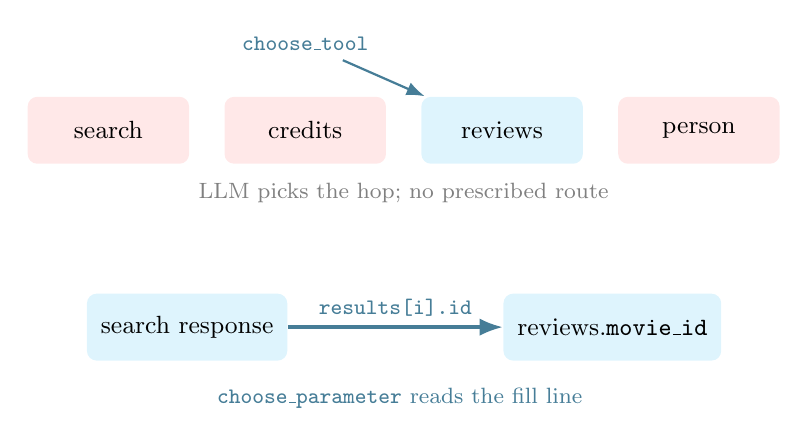
\begin{tikzpicture}[
  font=\small,
  catalog/.style={
    rounded corners=3.5pt, align=center, inner sep=5pt,
    minimum height=0.85cm, minimum width=2.05cm, fill=red!9
  },
  chosen/.style={
    rounded corners=3.5pt, align=center, inner sep=5pt,
    minimum height=0.85cm, minimum width=2.05cm, fill=cyan!13
  },
  pick/.style={-{Latex}, thick, cyan!55!black},
  fillarr/.style={-{Latex}, very thick, cyan!55!black}
]
\node[catalog] (search) at (0,1.35) {search};
\node[catalog] (credits) at (2.5,1.35) {credits};
\node[chosen] (reviews) at (5.0,1.35) {reviews};
\node[catalog] (person) at (7.5,1.35) {person};
\node[font=\footnotesize, cyan!55!black] (llm) at (2.5,2.45) {\texttt{choose\_tool}};
\draw[pick] (llm) -- (reviews);
\node[font=\footnotesize, gray] at (3.75,0.55) {LLM picks the hop; no prescribed route};

\node[chosen] (prod) at (1.0,-1.15) {search response};
\node[chosen] (cons) at (6.4,-1.15) {reviews.\texttt{movie\_id}};
\draw[fillarr] (prod) -- node[above, font=\footnotesize] {\texttt{results[i].id}} (cons);
\node[font=\footnotesize, cyan!55!black] at (3.7,-2.05) {\texttt{choose\_parameter} reads the fill line};
\end{tikzpicture}
\caption{The fill contract names a transition, not a route. \texttt{choose\_tool} still selects among catalog purposes. Once a hop is chosen, the guideline names the producer path of its path parameter and does not tell the model which sequence of APIs to call.}
\label{fig:transition}
\end{figure}

$D^\star$ is built from the vendor Initial dump. The frozen TMDB payload is fill, response, and $\mathrm{scope}(R_t)$. The frozen Spotify payload is fill plus a guideline response without sibling negation.

\FloatBarrier
\section{Experiments}

\subsection{Experiment setup}

\paragraph{Controller.}
Released DFSDT. $T{=}0.2$, $\mathrm{top\_p}{=}1$, $\mathrm{max\_tokens}{=}2000$, \texttt{retrieval\_num=5}.

\paragraph{Documents.}
DFSDT uses the vendor Initial catalog. DRAFT uses the released rewrite. Ours is the frozen compiled payload above (TMDB) and fill plus guideline response without sibling negation (Spotify).

\paragraph{Data and backends.}
RestBench-TMDB, $n{=}100$, live TMDB v3. RestBench-Spotify, $n{=}57$, live Spotify Web API, same controller. Gold paths are unchanged. Most Spotify gold paths start at user-account endpoints; the frozen map does not treat those calls as producers, so that split is not an execution contrast.

\paragraph{Metrics.}
Primary: execution-valid CP on finished TMDB cells. Secondary: ordered-path CP, the metric of RestGPT and DRAFT.

\paragraph{Models and seeds.}
Ling-3.0-Flash and DeepSeek V4, TMDB seeds $1$--$9$. Query-level labels flip across seeds, so intervals are seed-level Student-$t$ 95\% ($t_{8}{=}2.306$).

\subsection{Executable tool use}

\begin{table}[t]
\centering
\caption{Execution-valid CP (\%) on RestBench-TMDB. Seed-mean over 9 seeds, Student-$t$ 95\%. Bold is the best document on that model.}
\label{tab:exec}
\small
\begin{tabular}{lccc}
\toprule
Model & Initial & DRAFT & Ours \\
\midrule
Ling-3.0-Flash (9 seeds) & $51.0$ $[47.2,54.8]$ & $15.3$ $[12.7,18.0]$ & $\mathbf{57.0}$ $[53.9,60.2]$ \\
DeepSeek V4 (9 seeds) & $\mathbf{63.1}$ $[60.1,66.2]$ & $23.8$ $[21.5,26.1]$ & $62.2$ $[57.8,66.6]$ \\
\bottomrule
\end{tabular}
\end{table}

\begin{table}[t]
\centering
\caption{Paired seed-mean $\Delta$ in execution-valid CP, percentage points, TMDB.}
\label{tab:exec-delta}
\small
\begin{tabular}{lcc}
\toprule
Contrast & Ling (9 seeds) & DeepSeek V4 (9 seeds) \\
\midrule
Ours $-$ DRAFT & $\mathbf{+41.6\ [+36.6,+46.5]}$ & $\mathbf{+38.4}$\textsuperscript{*} \\
Ours $-$ Initial & $\mathbf{+6.0\ [+0.2,+11.8]}$ & $-0.9\ [-6.5,+4.7]$ \\
\bottomrule
\end{tabular}\\[2pt]
{\scriptsize *DeepSeek V4 vs DRAFT: every seed is positive; seed-mean gap $+38.7$ on triple-shared finished cells. Seed intervals are decode noise. A paired bootstrap over the 100 queries, seeds averaged inside a query: Ling Ours$-$Initial $+6.0$ $[+2.1,+10.0]$; DeepSeek V4 $-0.9$ $[-4.8,+3.0]$.}
\end{table}

On every Ling and DeepSeek V4 TMDB seed, Ours is above DRAFT on execution-valid CP (about $+42$ and $+39$\,pp). Ling also beats the catalog ($+6.0$\,pp); the query-level interval does not cover zero. DeepSeek V4 is on par with the catalog; DRAFT fails on both (15.3\% and 23.8\%). Per-seed values are in Appendix~\ref{app:seeds}.

\begin{figure}[H]
\centering
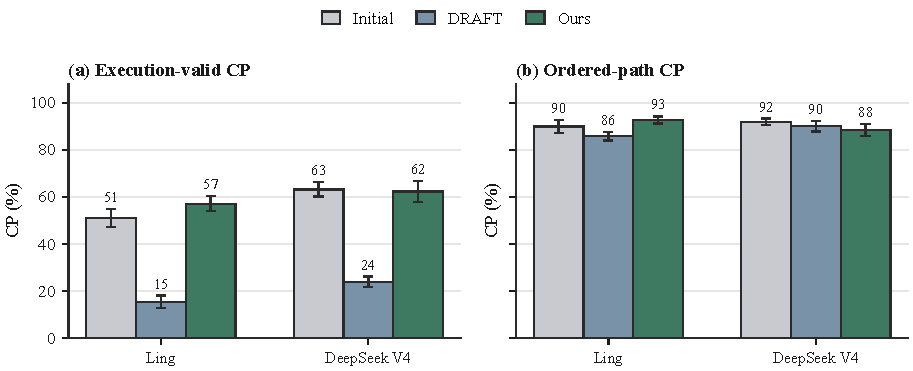
\includegraphics[width=\textwidth]{figures/results_tmdb.pdf}
\caption{RestBench-TMDB, same runs as Tables~\ref{tab:exec} and~\ref{tab:tmdb-cp}. Seed-mean over 9 seeds, Student-$t$ 95\% whiskers. (a)~Primary metric. (b)~Ordered-path CP.}
\label{fig:results-tmdb}
\end{figure}

DRAFT's descriptions look helpful and fill badly. Ordered-path CP can stay in the mid-80s to mid-90s while three-quarters of those traces fail HTTP (Table~\ref{tab:tmdb-cp}). DeepSeek V4 already executes well on the original catalog (63\%). Ours stays on par; DRAFT does not.

\begin{table}[t]
\centering
\caption{Seed-mean ordered-path CP (\%) on RestBench-TMDB. Same runs as Table~\ref{tab:exec}.}
\label{tab:tmdb-cp}
\small
\begin{tabular}{lccc}
\toprule
Model & Initial & DRAFT & Ours \\
\midrule
Ling-3.0-Flash & $89.9$ $[87.1,92.7]$ & $85.7$ $[83.9,87.4]$ & $\mathbf{92.7}$ $[91.1,94.2]$ \\
DeepSeek V4 & $\mathbf{91.9}$ $[90.4,93.3]$ & $90.0$ $[87.8,92.3]$ & $88.4$ $[85.8,91.0]$ \\
\bottomrule
\end{tabular}
\end{table}

\subsection{Sibling negation on DeepSeek V4}

On DeepSeek V4, Ours misses more first producers (35 vs 25 of 900) and more final consumers (49 vs 30) than Initial. The typical miss is not a wrong hop. Decompose has already named the gold consumer; \texttt{choose\_tool} then returns no valid choice because the catalog document contains \texttt{not GET\_<that consumer>}. Ling, on the same string, reads the negation as ``this search is not the credits call'' and still selects credits later. The fill line in the guideline is unchanged. That is why DeepSeek V4 stays on par with the catalog on execution-valid CP while ordered-path CP falls: the traces that survive selection still fill. Spotify search was compiled without sibling \texttt{not GET\_} names.

\subsection{Placement}
\label{sec:placement}

On TMDB Ling, one seed, putting path-parameter text into the schema plus a shared ``do not invent ids'' banner scored 80 CP with 10 first-API stuck queries. A hop gate in \texttt{choose\_tool} scored 82. Fill in the guideline only scored 93 with 2 stuck. Extra text in $u_t$ of hop APIs makes the agent repeat search. Response scope was therefore restricted to catalog $u_t$. Replacing the purpose with structural fingerprints collapses both models (Ling $36/48$, DeepSeek V4 $46/48$ on a frozen 24-query panel). Those two measurements are why fill stays in $d_t$ and why response scope is not written into hop $u_t$.

\begin{figure}[H]
\centering
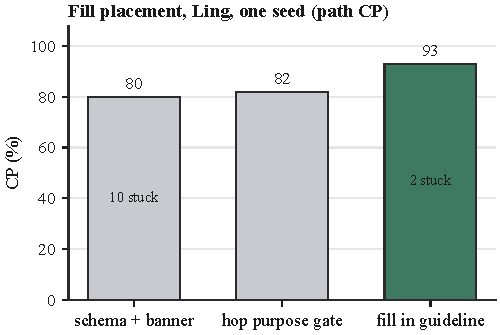
\includegraphics[width=0.72\textwidth]{figures/results_placement.pdf}
\caption{Where the fill line is written. Path CP, TMDB Ling, one seed. Grey bars are the two rejected slots; the green bar is the frozen write. Stuck counts are first-API repeats, reported only where that seed was counted.}
\label{fig:results-placement}
\end{figure}

\FloatBarrier
\section{Limitations}

The measured gain is a documentation effect inside the released DFSDT controller: the search procedure, the request schema, and the models stay fixed. The Spotify compiler does not bind user-account hops, so that split is not an execution contrast. Sibling negation on the TMDB catalog selection surface helps Ling and blocks DeepSeek V4; that is a limit of the same payload, not a second result. Ling and DeepSeek V4 TMDB runs used unpinned provider routing.

\section{Future work}

We will evaluate the same three documentation arms on ToolBench G3 instructions whose later required identifier is absent from the query and must be taken from an earlier response (Appendix~\ref{app:artifacts}). That setting asks the fill line to transform a payload, which RestBench-TMDB does not test. A third model family will be reported as a completed seed panel.

\section{Conclusion}

Vendor REST catalogs name the next endpoint and leave implicit how a later call should be filled from an earlier response. A free-form purpose rewrite can keep gold API names while the live call still fails. The intervention we can defend is a slot write inside DFSDT: a fill contract and a response contract in the guideline, hop purpose left as the vendor wrote it. That raises execution-valid CP on Ling relative to both the catalog and that rewrite. On DeepSeek V4 the same write matches the catalog and the rewrite fails. The fill line is the part that transfers; compressing sibling hops into \texttt{not GET\_} on the selection surface does not transfer across families.

\bibliographystyle{plainnat}
\bibliography{refs}

\appendix
\section{Worked examples}
\label{app:examples}

DRAFT prints a full documentation rewrite in its appendix; RestGPT prints gold paths next to the user question. We do the same for two RestBench-TMDB queries: the strings below are the frozen dumps, not a paraphrase.

\subsection{Search then credits}
\label{app:ex-credits}

Query~1: ``Who was the lead actor in the movie The Dark Knight?'' Gold path: \texttt{GET\_search\_movie}, \texttt{GET\_movie\_movie\_id\_credits}. The second URL is \texttt{/movie/\{movie\_id\}/credits}. Table~\ref{tab:ex-credits} is what each arm writes into the guideline $d_t$ of that hop. \texttt{choose\_tool} still sees the vendor purpose on the hop (``Get the cast and crew for a movie.''). The request schema is unchanged.

\begin{table}[H]
\centering
\caption{Guideline $d_t$ on \texttt{GET\_movie\_movie\_id\_credits} for query~1. DRAFT copies the same paragraph into $u_t$.}
\label{tab:ex-credits}
\small
\begin{tabular}{@{}l>{\raggedright\arraybackslash}p{0.72\textwidth}@{}}
\toprule
Arm & $d_t$ (hop) \\
\midrule
Initial & Get the cast and crew for a movie. \\
DRAFT & Prose rewrite of the same purpose. It says the movie ID is in the URL. It does not name a producer call or a JSON path. \\
Ours & Get the cast and crew for a movie. movie\_id from GET\_search\_movie, GET\_discover\_movie, GET\_movie\_popular, \ldots\ (results[i].id). Response: cast[i].credit\_id or crew[i].credit\_id. Downstream: GET\_credit\_credit\_id. \\
\bottomrule
\end{tabular}
\end{table}

The catalog search entry is one sentence (``Search for movies.''). Ours appends a response line to $d_t$ and a compressed scope line to $u_t$:

\begin{shaded}
\ttfamily\footnotesize
$d_t$: Response: results[i].\{id,title,release\_date,overview\}.\\
Downstream: GET\_movie\_movie\_id\_credits, GET\_movie\_movie\_id\_images, \ldots\\[0.3em]
$u_t$: Search for movies. Returns results[i].\{id,title,release\_date,overview\}.\\
not GET\_movie\_movie\_id\_credits, GET\_movie\_movie\_id\_images, \ldots
\end{shaded}

\subsection{Collection then review}
\label{app:ex-review}

Query~38 is Figure~\ref{fig:teaser}: ``Give me a review of a movie from the collection The Fast and the Furious.'' Gold path: \texttt{GET\_search\_collection}, \texttt{GET\_collection\_collection\_id}, \texttt{GET\_movie\_movie\_id\_reviews}. The last hop still needs a \texttt{movie\_id}. Collection detail is the producer of that id (\texttt{parts[i].id}); the reviews fill line still names search and list APIs, as in the closed map (Appendix~\ref{app:artifacts}).

\begin{table}[H]
\centering
\caption{Frozen strings on the two hops of query~38. Vendor changelog text on the collection page is omitted.}
\label{tab:ex-review}
\footnotesize
\begin{tabular}{@{}l>{\raggedright\arraybackslash}p{2.1cm}>{\raggedright\arraybackslash}p{0.58\textwidth}@{}}
\toprule
Hop & Slot & Written string \\
\midrule
search collection & $u_t$ Ours & Search for collections. Returns results[i].\{id,name\}. not GET\_collection\_collection\_id\_images, GET\_collection\_collection\_id. \\
search collection & $d_t$ Ours & Search for collections. Response: results[i].\{id,name\}. Downstream: GET\_collection\_collection\_id\_images, GET\_collection\_collection\_id. \\
collection by id & $d_t$ Ours & collection\_id from GET\_search\_collection (results[i].id). Response: id, name, parts[i].id, production\_companies. \\
movie reviews & $d_t$ Initial & Get the user reviews for a movie. \\
movie reviews & $d_t$ DRAFT & ``This API retrieves user reviews for a specific movie using the movie ID included in the URL path as a required parameter \ldots'' Copied into $u_t$. An attached example uses movie ID 11111. \\
movie reviews & $d_t$ Ours & movie\_id from GET\_search\_movie, GET\_discover\_movie, GET\_movie\_popular, \ldots\ (results[i].id). Response: results[i].id. Downstream: GET\_review\_review\_id. \\
\bottomrule
\end{tabular}
\end{table}

Under Initial the collection id can be filled while \texttt{movie\_id} stays a stub; HTTP rejects the review call. Under DRAFT both stubs stay empty. Under Ours the controller reads \texttt{parts[i].id} from the collection payload and the review call returns a user review.

\section{Per-seed TMDB results}
\label{app:seeds}

Tables~\ref{tab:exec} and~\ref{tab:exec-delta} report seed means. Tables~\ref{tab:seed-ling} and~\ref{tab:seed-flash} are the nine TMDB seeds that enter those means. A leftover driver or transport error is a miss and stays in the denominator. Seeds are $1$--$9$ ($T{=}0.2$). No seed is dropped.

\begin{table}[H]
\centering
\caption{Execution-valid CP (\%) on RestBench-TMDB, Ling-3.0-Flash, one seed per row.}
\label{tab:seed-ling}
\small
\begin{tabular}{cccc}
\toprule
Seed & Initial & DRAFT & Ours \\
\midrule
1 & 50.0 & 14.0 & 58.0 \\
2 & 47.0 & 10.0 & 65.0 \\
3 & 50.0 & 17.0 & 62.0 \\
4 & 55.0 & 21.0 & 54.0 \\
5 & 53.0 & 18.0 & 54.0 \\
6 & 57.0 & 16.0 & 54.0 \\
7 & 41.0 & 11.0 & 56.0 \\
8 & 50.0 & 14.0 & 53.0 \\
9 & 56.0 & 17.0 & 57.0 \\
\midrule
Mean & 51.0 & 15.3 & 57.0 \\
\bottomrule
\end{tabular}
\end{table}

\begin{table}[H]
\centering
\caption{Execution-valid CP (\%) on RestBench-TMDB, DeepSeek V4, one seed per row.}
\label{tab:seed-flash}
\small
\begin{tabular}{cccc}
\toprule
Seed & Initial & DRAFT & Ours \\
\midrule
1 & 63.0 & 24.0 & 53.0 \\
2 & 55.0 & 23.0 & 64.0 \\
3 & 63.0 & 22.0 & 67.0 \\
4 & 66.0 & 20.0 & 58.0 \\
5 & 67.0 & 29.0 & 59.0 \\
6 & 59.0 & 24.0 & 61.0 \\
7 & 67.0 & 27.0 & 59.0 \\
8 & 65.0 & 25.0 & 68.0 \\
9 & 63.0 & 20.0 & 71.0 \\
\midrule
Mean & 63.1 & 23.8 & 62.2 \\
\bottomrule
\end{tabular}
\end{table}

Ours is above DRAFT on every seed of both families. Against Initial, Ling is above on seven of nine seeds and DeepSeek V4 on five of nine. That is the decode-level spread behind the seed-mean intervals, not a second experiment.

\section{Artifacts and protocol}
\label{app:artifacts}

\subsection{Bind versus gold paths}
\label{app:bind}

Bind is a closed map over the 54-API TMDB dump. It does not read RestBench gold paths. Table~\ref{tab:bind-gold} is a post-hoc audit: for each gold hop that is not the first call, whether some closed-map producer already appears earlier on that gold path.

\begin{table}[H]
\centering
\caption{Closed-map producers on RestBench-TMDB gold paths. 122 gold hops that are not the first call.}
\label{tab:bind-gold}
\small
\begin{tabular}{lc}
\toprule
Gold hop (not first) & Count \\
\midrule
At least one closed-map producer earlier on the path & 91 \\
Needs an intermediate hop as the producer & 31 \\
\bottomrule
\end{tabular}
\end{table}

The 31 residual hops take \texttt{person\_id} from movie credits, \texttt{movie\_id} from a person's credit list, or \texttt{season\_number} from a TV object. The fill line still names search and list APIs. The overlap is an audit, not a training signal.

\subsection{DRAFT slots}
\label{app:draft-slots}

The released TMDB DRAFT dump has one \texttt{description} field and no separate \texttt{tool\_description}. The DFSDT adapter copies that field into both $u_t$ and $d_t$ on all 54 tools. Every hop also carries an \texttt{example}; seven of those examples use the invented identifiers 11111 or 13579. Table~\ref{tab:ex-review} quotes one. DRAFT's 15.3\% execution-valid CP is not an empty guideline. It is a purpose rewrite, with fake identifiers, in both slots.

\subsection{Named-entity identifiers}
\label{app:gold-id}

Execution-valid CP accepts any HTTP-valid path id. A second check freezes named-entity ids once (Titanic, Sofia Coppola, Star Wars collection parts) and, on popular and trending gold paths, harvests ids from the producer of that trace.

\begin{table}[H]
\centering
\caption{Named-id CP (\%), same TMDB traces as Table~\ref{tab:exec}. Query-level Ours$-$Initial on Ling is $+2.0$ $[-0.9,+4.9]$ and covers zero.}
\label{tab:named-id}
\small
\begin{tabular}{lccc}
\toprule
Model & Initial & DRAFT & Ours \\
\midrule
Ling-3.0-Flash & 40.2 & 12.0 & 42.2 \\
DeepSeek V4 & 50.2 & 20.3 & 48.9 \\
\bottomrule
\end{tabular}
\end{table}

The fill line repairs stubs against DRAFT. On this freeze it does not beat the catalog at picking the named title.

\subsection{Probe seeds}
\label{app:probe}

The frozen TMDB payload records \texttt{examples\_from\_probe=0} and empty \texttt{seed\_ids}. No probe token was written into $d_t$. The five titles reserved for a probe, had one run, were Inception, Game of Thrones, Tom Hanks, Disney, and Star Wars. None of those strings occur in \texttt{TMDB\_Ours.json}. Query~38 uses The Fast and the Furious; that title is not a seed.

\subsection{ToolBench G3 nested slice}
\label{app:g3}

Released G3 has 100 instructions. Table~\ref{tab:g3} splits them by whether a later required identifier is already in the user text. Indices: \texttt{artifacts/documentation/G3\_nested.json}.

\begin{table}[H]
\centering
\caption{Released ToolBench G3 instructions, $n{=}100$.}
\label{tab:g3}
\small
\begin{tabular}{lc}
\toprule
Slice & Count \\
\midrule
Nested: later required id absent from the query & 40 \\
Independent: every gold identifier already in the query & 39 \\
Underspecified: an identifier is missing and no earlier gold API & 21 \\
\bottomrule
\end{tabular}
\end{table}

\subsection{Reproducibility}

Contracts are compiled by \texttt{src/tooldoc\_nir/restbench\_ours.py}.
The released DFSDT controller is driven by \texttt{python -m tooldoc\_nir.restbench\_table}.
Decoding is $T{=}0.2$, $\mathrm{top\_p}{=}1$, $\mathrm{max\_tokens}{=}2000$, \texttt{retrieval\_num=5}.
Traces live under \texttt{artifacts/results/}. Vendor keys stay in a local \texttt{.env}.

\end{document}
